\documentclass{article}
\usepackage[UTF8]{ctex}                     % 支持中文显示
\usepackage{CJKutf8}
\usepackage{amsmath}
\usepackage{listings}
\usepackage{color} %red, green, blue, yellow, cyan, magenta, black, white
\usepackage{xcolor}
\usepackage{graphicx}
\definecolor{mygreen}{RGB}{28,172,0} % color values Red, Green, Blue
\definecolor{mylilas}{RGB}{170,55,241}
\lstset{language=Python,%
    %basicstyle=\color{red},
    breaklines=true,%
    morekeywords={imread},
    keywordstyle=\color{blue},%
    morekeywords=[2]{1}, keywordstyle=[2]{\color{black}},
    identifierstyle=\color{black},%
    stringstyle=\color{mylilas},
    commentstyle=\color{mygreen},%
    showstringspaces=false,%without this there will be a symbol in the places where there is a space
    numbers=left,%
    numberstyle={\color{black!40}},% size of the numbers
    numbersep=9pt, % this defines how far the numbers are from the text
    emph=[1]{for,end,break},emphstyle=[1]\color{red}, %some words to emphasise
    %emph=[2]{word1,word2}, emphstyle=[2]{style},
    escapeinside=``
}




\begin{document}
\begin{CJK*}{UTF8}{song}

\title{{图像处理-作业一}}
\author{刘书裴}
\date{\today}
\maketitle

\section{绘制{[}0,2pi{]}上y1=sinx,y2=cosx,y3=x\^{}2曲线在同一张图片中}

1) 思路一

所用语言:python3

所用库:PIL,numpy

思路:初始化X数组,分别计算出Y1、Y2、Y3,新建指定大小的二维数组后按比例插值,最后将二维数组转为图片输出。

代码:

\begin{lstlisting}
from PIL import Image
import numpy as np

def generateFigure(shape=(256, 256), thickness=1):
    step = 2 * np.pi / shape[0]
    X = np.arange(0, 2 * np.pi + step, step)
    Y1, Y2, Y3 = np.sin(X), np.cos(X), X ** 2
    MAX = shape[1] // 2
    img = np.zeros((shape[1], shape[0], 3), dtype=np.uint8)
    for i in range(shape[0]):
        for t in range(-thickness // 2, thickness // 2, 1):
            y1, y2, y3 = int(Y1[i] / step) + t, int(Y2[i] / step) + t, int(Y3[i] / step) + t
            if np.abs(y1) < MAX:
                img[-y1 + MAX, i, 0] = 255 - np.abs(t) / thickness * 256
            if np.abs(y2) < MAX:
                img[-y2 + MAX, i, 1] = 255 - np.abs(t) / thickness * 256
            if np.abs(y3) < MAX:
                img[-y3 + MAX, i, 2] = 255 - np.abs(t) / thickness * 256
    img = Image.fromarray(img)
    img.show()
    img.save(r"./result/homework1_1.jpg")
\end{lstlisting}

结果:

\begin{figure}[htbp]
    \centering
    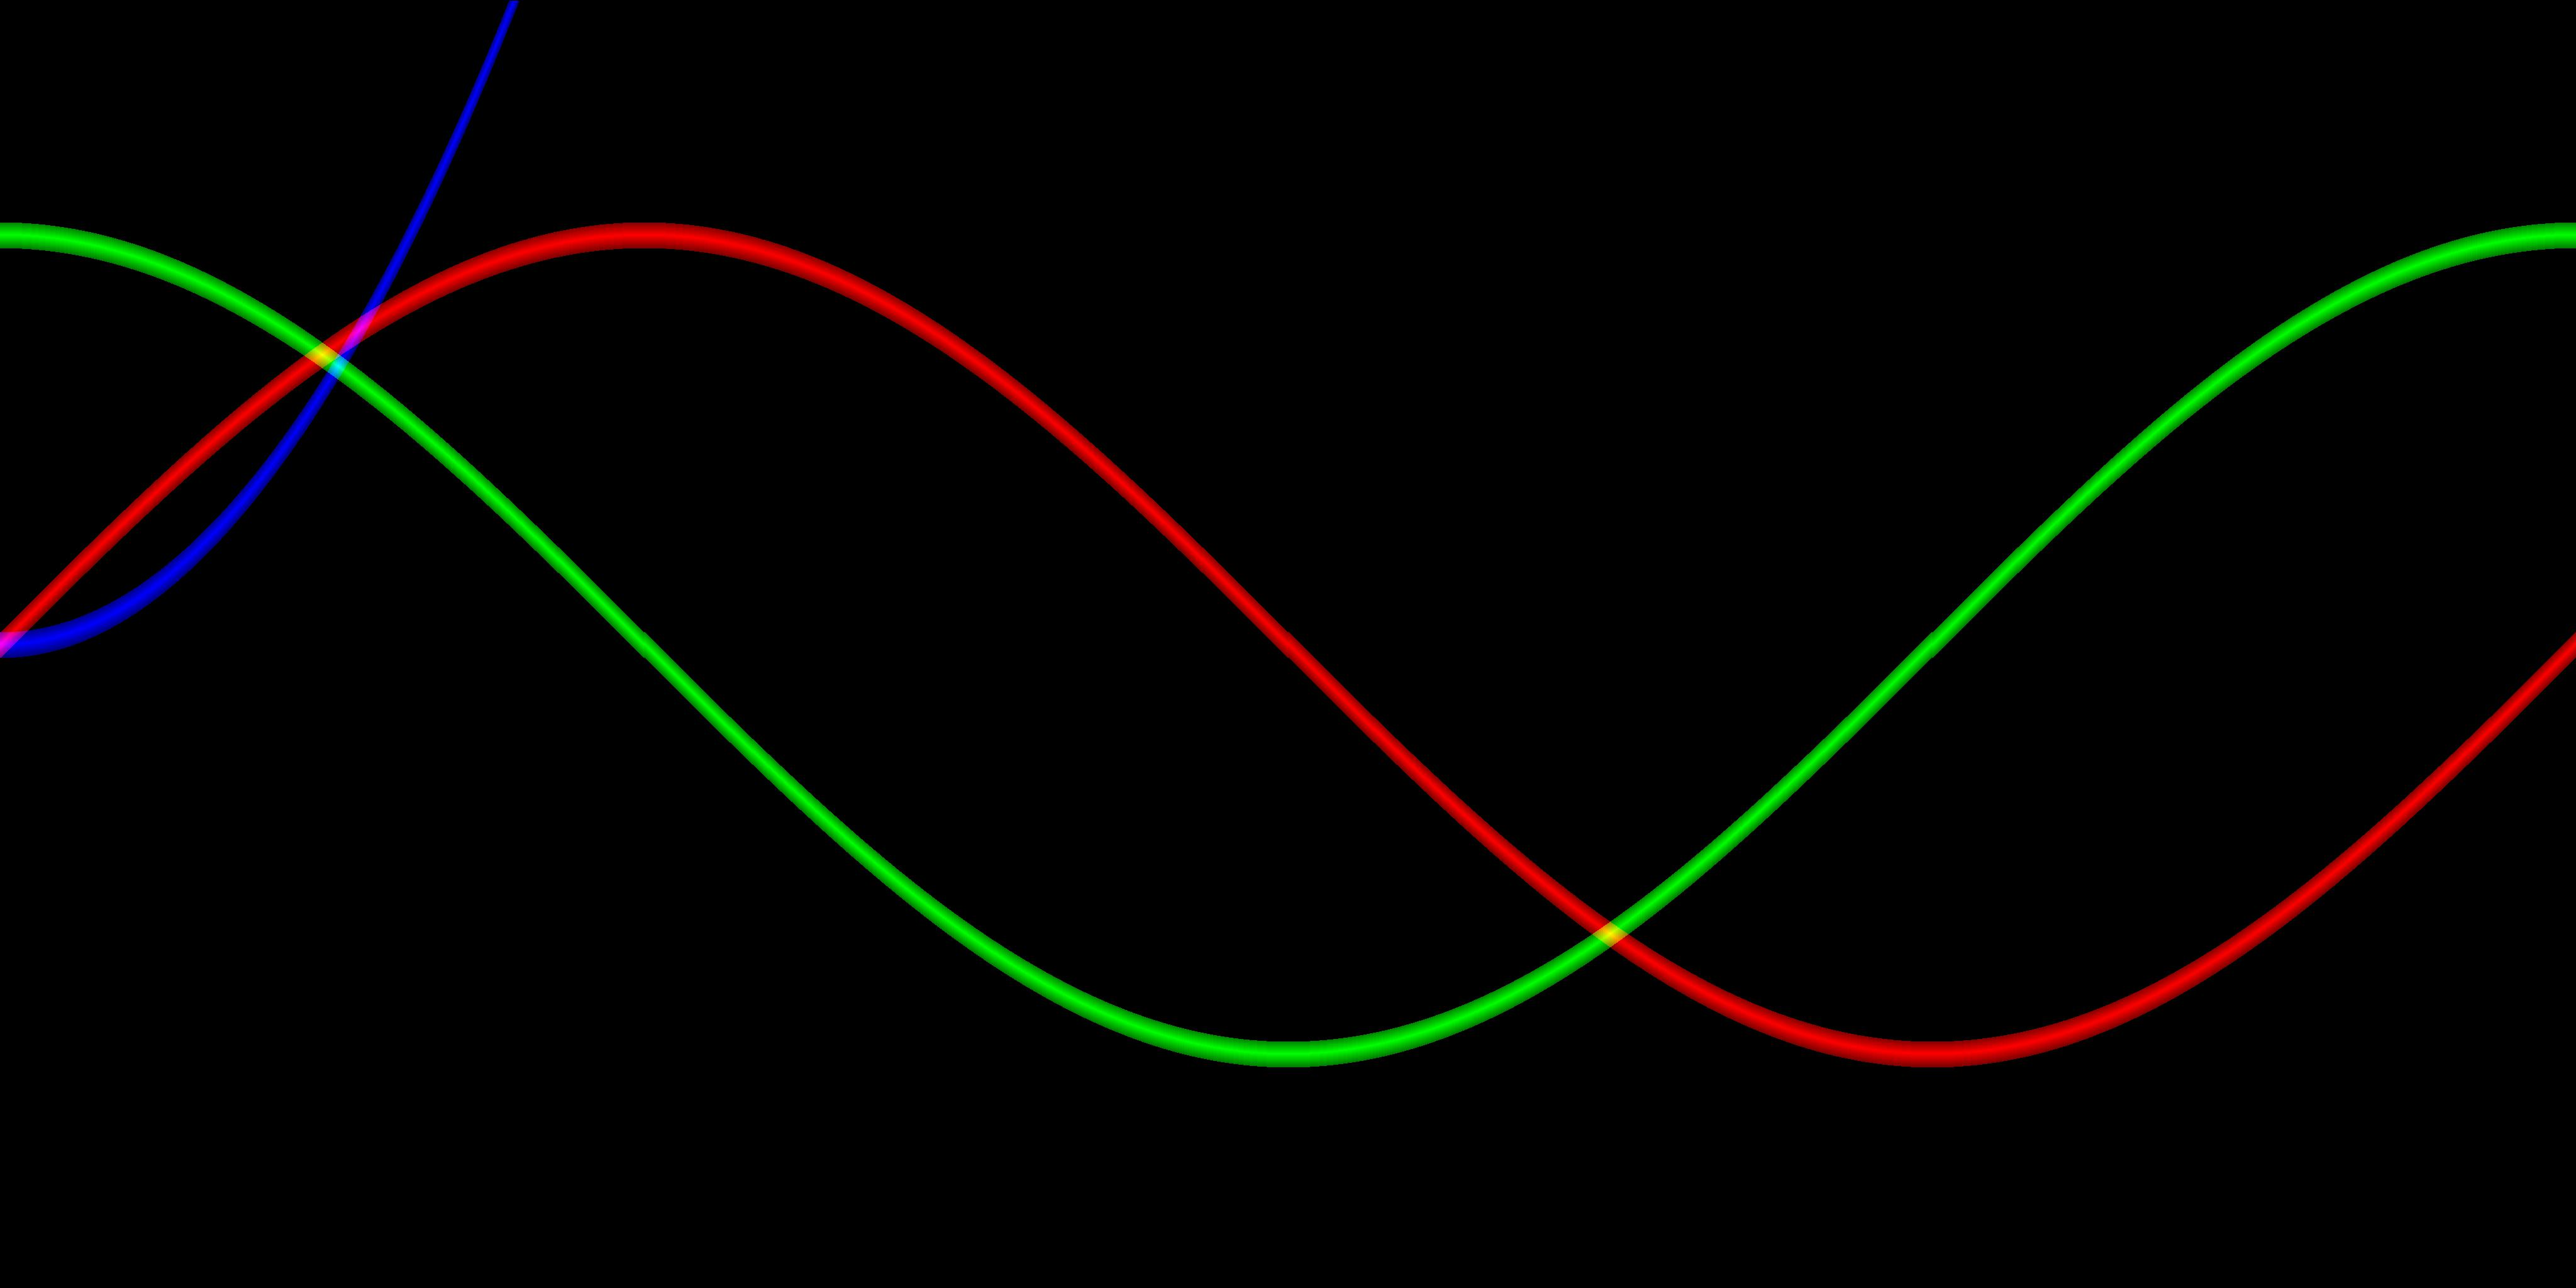
\includegraphics[width=0.8\linewidth]{result/homework1_1.jpg}
    \caption{result1}
\end{figure}

2) 思路二

所用语言:python3

所用库:matplotlib,numpy

思路:初始化X数组,分别计算出Y1、Y2、Y3,直接使用matplotlib库绘制曲线。

代码:

\begin{lstlisting}
import numpy as np
from matplotlib import pyplot as plt

def generateFigure2():
    X = np.arange(0, 2 * np.pi, 0.001)
    Y1, Y2, Y3 = np.sin(X), np.cos(X), X ** 2
    plt.plot(X, Y1, 'r', label="y=sinx")
    plt.plot(X, Y2, 'g', label="y=cosx")
    plt.plot(X, Y3, 'b', label="y=x^2")
    plt.xlabel("X")
    plt.ylabel("Y")
    plt.legend()
    plt.savefig(r"./result/homework1_2.jpg")
    plt.show()
\end{lstlisting}

结果:

\begin{figure}[htbp]
    \centering
    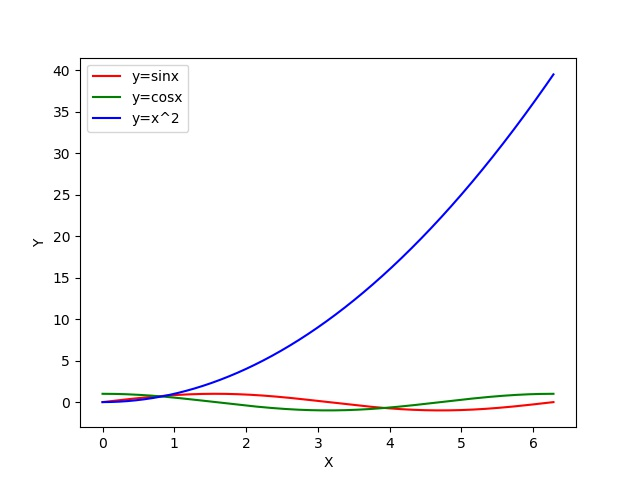
\includegraphics[width=0.9\linewidth]{result/homework1_2.jpg}
    \caption{result2}
\end{figure}

\section{不使用for的双线性插值}

除了调包,否则不可能实现不使用for的双线性插值。

能力有限,只能实现普通的双线性插值(未调包),详情见

\href{https://github.com/3017218062/Image-Super-Resolution/tree/master/interpolation}

\end{CJK*}
\end{document}